\section{Einführung}
\section{Versuch}
Im Folgendem werden die Kennlienen von verschieden Bauteilen mit dem Aufbau~\ref{fig:aufbau} bestimmt. Sämtliche Messwerte für die Spannung wurden mit einem Messfehler von $\Delta U = V$ bzw. $\Delta I = mA$ aufgenommen.
\begin{figure}[H]
	\centering
	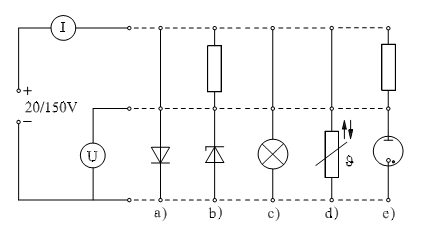
\includegraphics[width=.8\textwidth]{Aufbau.png}
	\caption{Messaufbau für unterschiedliche Leiter}
	\label{fig:aufbau}
\end{figure}
\subsection{Diode in Durchlassrichtung}
Wie in Abbildung~\ref{fig:aufbau} a) gezeigt wird der Strom für unterschiedliche Spannung gemessen, um daraus eine U-I-Kennlinie zu ermitteln.

\begin{figure}[H]
\centering
\begin{tikzpicture}
  \begin{axis}[
    width=15 cm,
    height=9 cm,
    xmin=0, xmax=0.8,
    ymin=-1, ymax=60,
    xlabel={$U$ [\si{mV}]},
    ylabel={$I$ [\si{mA}]},
    domain=0:0.8,
    cycle list name=color list,
    legend entries={Messwerte, $a\cdot b^x$},
    legend pos=north west
  ]
  \addplot+ plot [only marks,mark=x, error bars/.cd, x dir=both, x fixed=0.002, y dir=both, y explicit]  table[y error index=2] {Diode.txt};
  \addplot+ plot [samples=200, mark=none] {5.61784*10^(-7)*(1.69598*10^11)^x};
  \end{axis}
\end{tikzpicture}
\caption{Messwerte und Fit für eine Diode in Durchlassrichtung}
\label{fig:diode}
\end{figure}
Die Fehlerbalken sind sehr kurz und deshalb schwer zu erkennen.

Aufgrund des anscheinend exponentiellen Verlaufs der Messwerte wurde mit \emph{gnuplot} nach dem \emph{least-squares}-Verfahren die Werte gegen die Funktion $f(x)=a\cdot b^x$ gefittet. Ausgabe:
\begin{table}[H]
  \centering
  \begin{tabular}{c | c | c }
    Variable  & Wert & Unsicherheit\\ \hline
    a & $\num{5.61784d-7}$ & $\pm\num{3.084d-8}$ \\
    b & $\num{1.69598d+11}$ & $\pm\num{1.319d+10}$
  \end{tabular}
  \caption{Linearer Fit zu Abbildung~\ref{fig:diode}}
  \label{tab:fitdiode}
\end{table}
\subsection{Zenerdiode}
Wie in Abbildung~\ref{fig:aufbau} b) gezeigt wird der Strom für unterschiedliche Spannung gemessen, um daraus eine U-I-Kennlinie zu ermitteln. Dies wird jedoch einmal mit einer Polung in Durchlassrichtung und einmal in Sperrrichtung getan.
\begin{figure}[H]
\centering
\begin{tikzpicture}
  \begin{axis}[
    width=15 cm,
    height=9 cm,
    xmin=0, xmax=6,
    ymin=-1, ymax=30,
    xlabel={$U$ [\si{V}]},
    ylabel={$I$ [\si{mA}]},
    domain=0:6,
    cycle list name=color list,
    legend entries={Messwerte, $a\cdot b^x$},
    legend pos=north west
  ]
  \addplot+ plot [only marks,mark=x, error bars/.cd, x dir=both, x fixed=0.002, y dir=both, y explicit]  table[y error index=2] {Diodesperr.txt};
  \addplot+ plot [samples=200, mark=none] {1.50271*10^(-7)*(42.7533)^x};
  \end{axis}
\end{tikzpicture}
\caption{Messwerte und Fit für eine Zenerdiode in Sperrrichtung}
\label{fig:diodesperr}
\end{figure}
Die Fehlerbalken sind sehr kurz und deshalb schwer zu erkennen.

Aufgrund des anscheinend exponentiellen Verlaufs der Messwerte wurde mit \emph{gnuplot} nach dem \emph{least-squares}-Verfahren die Werte gegen die Funktion $f(x)=a\cdot b^x$ gefittet. Ausgabe:
\begin{table}[H]
  \centering
  \begin{tabular}{c | c | c }
    Variable & Wert & Unsicherheit\\ \hline
    a & $\num{1.50271d-7}$ & $\pm\num{5.433d-8}$ \\
    b & $\num{42.7533}$ & $\pm\num{3.073}$
  \end{tabular}
  \caption{Linearer Fit zu Abbildung~\ref{fig:diodesperr}}
  \label{tab:fitdiodesperr}
\end{table}
\begin{figure}[H]
\centering
\begin{tikzpicture}
  \begin{axis}[
    width=15 cm,
    height=9 cm,
    xmin=0, xmax=0.8,
    ymin=-1, ymax=40,
    xlabel={$U$ [\si{V}]},
    ylabel={$I$ [\si{mA}]},
    domain=0:0.8,
    cycle list name=color list,
    legend entries={Messwerte, $a\cdot b^x$},
    legend pos=north west
  ]
  \addplot+ plot [only marks,mark=x, error bars/.cd, x dir=both, x fixed=0.002, y dir=both, y explicit]  table[y error index=2] {Diodedurch.txt};
  \addplot+ plot [samples=200, mark=none] {3.08803*10^(-11)*(9.72068*10^16)^x};
  \end{axis}
\end{tikzpicture}
\caption{Messwerte und Fit für eine Zenerdiode in Durchlassrichtung}
\label{fig:diodedurch}
\end{figure}
Die Fehlerbalken sind sehr kurz und deshalb schwer zu erkennen.

Aufgrund des anscheinend exponentiellen Verlaufs der Messwerte wurde mit \emph{gnuplot} nach dem \emph{least-squares}-Verfahren die Werte gegen die Funktion $f(x)=a\cdot b^x$ gefittet. Ausgabe:
\begin{table}[H]
  \centering
  \begin{tabular}{c | c | c }
    Variable & Wert & Unsicherheit\\ \hline
    a & $\num{3.08803d-11}$ & $\pm\num{3.759d-12}$ \\
    b & $\num{9,72068d16}$ & $\pm\num{1.673d16}$
  \end{tabular}
  \caption{Linearer Fit zu Abbildung~\ref{fig:diodedurch}}
  \label{tab:fitdiodedurch}
\end{table}
\subsection{Glühlampe}
Wie in Abbildung~\ref{fig:aufbau} c) gezeigt wird der Strom für unterschiedliche Spannung gemessen, um daraus eine U-I-Kennlinie zu ermitteln.

\begin{figure}[H]
\centering
\begin{tikzpicture}
  \begin{axis}[
    width=15 cm,
    height=9 cm,
    xmin=0, xmax=14,
    ymin=0, ymax=60,
    xlabel={$U$ [\si{V}]},
    ylabel={$I$ [\si{mA}]},
    domain=0:14,
    cycle list name=color list,
    legend entries={Messwerte, $a\sqrt{x}$},
    legend pos=north west
  ]
  \addplot+ plot [only marks,mark=x, error bars/.cd, x dir=both, x fixed=0.002, y dir=both, y explicit]  table[y error index=2] {Lampe.txt};
  \addplot+ plot [samples=200, mark=none] {14.9315*sqrt(x)};
  \end{axis}
\end{tikzpicture}
\caption{Messwerte und Fit für eine Lampe}
\label{fig:Lampe}
\end{figure}
Die Fehlerbalken sind sehr kurz und deshalb schwer zu erkennen.

Aufgrund des anscheinend Wurzel-artigem Verlaufs der Messwerte, besonders im Bereich bis $3V$, wurde mit \emph{gnuplot} nach dem \emph{least-squares}-Verfahren die Werte gegen die Funktion $f(x)=a\cdot\sqrt{x}$ gefittet. Ausgabe:
\begin{table}[H]
  \centering
  \begin{tabular}{c | c | c }
    Variable & Wert & Unsicherheit\\ \hline
    a & $\num{14,9315}$ & $\pm\num{0,2092}$ \\
   
  \end{tabular}
  \caption{Linearer Fit zu Abbildung~\ref{fig:Lampe}}
  \label{tab:fitlampe}
\end{table}
\subsection{NTC}
Wie in Abbildung~\ref{fig:aufbau} d) gezeigt wird der Strom für unterschiedliche Spannung gemessen, um daraus eine U-I-Kennlinie zu ermitteln. Dabei muss nach jeder Spannungserhöhung gewartet werden, bis sich der Temperaturgradient abgebaut hat. 

\begin{figure}[H]
\centering
\begin{tikzpicture}
  \begin{axis}[
    width=15 cm,
    height=9 cm,
    xmin=0, xmax=8,
    ymin=0, ymax=60,
    xlabel={$U$ [\si{V}]},
    ylabel={$I$ [\si{mA}]},
    domain=0:8,
    cycle list name=color list,
    legend entries={Messwerte, $ax^2+bx+c$},
    legend pos=north west
  ]
  \addplot+ plot [only marks,mark=x, error bars/.cd, x dir=both, x fixed=0.01, y dir=both, y explicit]  table[y error index=2] {NTC1.txt};
  \addplot+ plot [samples=200, mark=none] {0.316693*x^2-0.0533435*x+1.05214};
  \end{axis}
\end{tikzpicture}
\caption{Messwerte und Fit für eine NTC-Widerstand}
\label{fig:ntc}
\end{figure}
Die Fehlerbalken sind sehr kurz und deshalb schwer zu erkennen.

Aufgrund des anscheinend quadratischem Verlaufs der Messwerte wurde mit \emph{gnuplot} nach dem \emph{least-squares}-Verfahren die Werte gegen die Funktion $f(x)=a\cdot x^2+b\cdot x+c$ gefittet. Beim Fitten wurde der letzte Messwert nicht betrachtet, da er vollkommen aus dem Verlauf der Werte herausfällt. Dies ist auf ein Versagen der Leistung des Netzgeräts zurückzuführen. Ausgabe:
\begin{table}[H]
  \centering
  \begin{tabular}{c | c | c }
    Variable   & Wert & Unsicherheit\\ \hline
    a & $\num{0,316693}$ & $\pm\num{0,05691}$ \\
    b & $\num{-0,0533435}$ & $\pm\num{0,4446}$ \\
    c & $\num{1,05214}$ & $\pm\num{0,6146}$ \\
  \end{tabular}
  \caption{Quadratischer Fit zu Abbildung~\ref{fig:ntc}}
  \label{tab:fitntc}
\end{table}
\subsection{Glimmlampe}
Wie in Abbildung~\ref{fig:aufbau} e) gezeigt wird der Strom für unterschiedliche Spannnungen gemessen. Dabei wird zuerst durch langsames Hochdrehen der Spannung bis zur Zündung der Lampe die Zündspannung bestimmt. Anschließend wird die Spannung langsam reduziert, bis die Glimmlampe erlischt, um die Löschspannung zu bestimmen. Wir erhalten als Mittelwerte für jeweils drei Messungen:
\begin{table}[H]
  \centering
  \begin{tabular}{c | c}
    Zündspannung & \SI{112.0(1)}{V} \\ \hline
    Löschspannung & \SI{83.3(1)}{V} \\
  \end{tabular}
  \caption{Messergebnis zur Glimmlampe}
  \label{tab:glimm}
\end{table}

Anschließend messen wir den Strom von der höchstmöglichen bis zur Löschspannung durch:

\begin{figure}[H]
\centering
\begin{tikzpicture}
  \begin{axis}[
    width=15 cm,
    height=9 cm,
    xmin=83.2, xmax=86.9,
    ymin=1.2, ymax=15.8,
    xlabel={$U$ [\si{V}]},
    ylabel={$I$ [\si{mA}]},
    domain=83.2:86.9,
    cycle list name=color list,
    legend entries={Messwerte, $ax+b$},
    legend pos=north west
  ]
  \addplot+ plot [only marks,mark=x, error bars/.cd, x dir=both, x fixed=0.1, y dir=both, y fixed=0.02]  table {glimm.txt};
  \addplot+ plot [mark=none] {3.93146*x-325.67};
  \end{axis}
\end{tikzpicture}
\caption{Messwerte für die Glimmlampe}
\label{fig:glimm}
\end{figure}
Aufgrund des anscheinend linearen Verlaufs der Messwerte wurde mit \emph{gnuplot} nach dem \emph{least-squares}-Verfahren die Werte gegen die Funktion $f(x)=a\cdot x +b$ gefittet. Ausgabe:
\begin{table}[H]
  \centering
  \begin{tabular}{c | c | c }
    Variable   & Wert & Unsicherheit\\ \hline
    a & $\num{3.93146}$ & $\pm\num{0.07344}$ \\
    b & $\num{-325.67}$ & $\pm\num{6.243}$ \\
  \end{tabular}
  \caption{Linearer Fit zu Abbildung \ref{fig:glimm}}
  \label{tab:fitglimm}
\end{table}
\subsection{Temperaturabhängigkeit des Widerstandes eines Metalldrahtes}
Der Zusammenhang aus der Theorie gilt für den spezifischen Widerstand $\rho$, jedoch messen wir im Versuch den Widerstand $R=\rho\cdot l/A$, wobei $l$ die Länge des Leiters und $A$ die Querschnittsfläche ist. Wir gehen näherungsweise davon aus, dass die thermische Ausdehnung während des Versuches gering ist und nehmen deshalb $l$ und $A$ als konstant an. Für den Fit definieren wir $C\coloneqq \rho_0\cdot l/A$.

Die Messwerte werden für Aufheizen bzw. Abkühlen getrennt mit \emph{gnuplot} nach dem \emph{least-squares}-Verfahren gegen die aus der Theorie erwartete Funktion $R(T)=C(1+\alpha\cdot T$ gefittet. 
\begin{figure}[H]
\centering
\begin{tikzpicture}
  \begin{axis}[
    width=15 cm,
    height=9 cm,
    xmin=22, xmax=90,
    ymin=5.5, ymax=7,
    xlabel={$T$ [\si{\degreeCelsius}]},
    ylabel={$R$ [\si{\ohm}]},
    domain=22:90,
    cycle list name=color list,
    legend entries={Messwerte, $C_{\text{auf}}(1+\alpha_{\text{auf}}\cdot T)$},
    legend pos=north west
  ]
  \addplot+ plot [only marks,mark=x, error bars/.cd, x dir=both, x fixed=2, y dir=both, y fixed=0.126]  table {aufheizen.txt};
  \addplot+ plot [mark=none] {5.06455*(1+0.00448047*x)};
  \end{axis}
\end{tikzpicture}
\caption{Messwerte und Fit fürs Aufheizen}
\label{fig:aufheizen}
\end{figure}

\begin{table}[H]
  \centering
  \begin{tabular}{c | c}
    Variable & Wert \\ \hline
    $C_{\text{auf}}$ & $\SI{5.06455(3523)}{\ohm}$ \\
    $\alpha_{\text{auf}}$ & $\SI{4.48047(16030)}{\milli\ohm\per\degreeCelsius}$ \\
  \end{tabular}
  \caption{Fit zu Abbildung~\ref{fig:aufheizen}}
  \label{tab:fitaufheizen}
\end{table}
\begin{figure}[H]
\centering
\begin{tikzpicture}
  \begin{axis}[
    width=15 cm,
    height=9 cm,
    xmin=24, xmax=89,
    ymin=5.5, ymax=7,
    xlabel={$T$ [\si{\degreeCelsius}]},
    ylabel={$R$ [\si{\ohm}]},
    domain=24:87,
    cycle list name=color list,
    legend entries={Messwerte, $C_{\text{ab}}(1+\alpha_{\text{ab}}\cdot T)$},
    legend pos=north west
  ]
  \addplot+ plot [only marks,mark=x, error bars/.cd, x dir=both, x fixed=2, y dir=both, y fixed=0.126]  table {abkuehlen.txt};
  \addplot+ plot [mark=none] {5.06929*(1+0.00430956*x)};
  \end{axis}
\end{tikzpicture}
\caption{Messwerte und Fit fürs Abkühlen}
\label{fig:abkuehlen}
\end{figure}
\begin{table}[H]
  \centering
  \begin{tabular}{c | c}
    Variable & Wert \\ \hline
    $C_{\text{ab}}$ & $\SI{5.06929(2510)}{\ohm}$ \\
    $\alpha_{\text{ab}}$ & $\SI{4.30956(10240)}{\milli\ohm\per\degreeCelsius}$ \\
  \end{tabular}
  \caption{Fit zu Abbildung~\ref{fig:abkuehlen}}
  \label{tab:fitabkuehlen}
\end{table}
\section{Diskussion}
\notecite{anleitung-ws2014}
